% Analisi dei requisiti

\chapter{Analisi dei requisiti}\label{chap:requirements}

\section{Attori coinvolti}
Gli attori attivi nei vari scenari dei casi d'uso individuati sono quattro, di 
cui tre principali e uno secondario.
\subsection{Attori principali}
\subsubsection{Utente Zimbra}
L'applicazione è destinata solamente agli utenti Zimbra. Ciò si traduce nel 
fatto che si può accedere alle funzionalità di Teamwork solo se si è già in 
possesso di un'email Zimbra gestita dai loro server.  
\subsubsection{Utente OpenChat}
Un utente OpenChat, specializzazione dell'utente Zimbra, rappresenta un utente che utilizza un'istanza di Zimbra con la zimlet OpenChat installata. Questa zimlet permette di chattare con gli utenti Zimbra dello stesso server.

\subsubsection{Utente Teamwork web}
Un utente Teamwork web, specializzazione dell'utente OpenChat, rappresenta 
un utente che, oltre ad utilizzare un'istanza di Zimbra con la zimlet OpenChat, 
ha installato anche la zimlet Teamwork, applicazione di chat potenziata rispetto 
a OpenChat disponibile solo per la suite Zextras.

\subsection{Attori secondari}
\subsubsection{Server Zimbra}
Un server Zimbra è un'istanziazione della suite di prodotti Zimbra e, in caso, 
dei prodotti Zextras. Tramite esso si accede a tutti i dati del profilo Zimbra 
così da mantenerli sincronizzati tra le varie sessioni in uso.

\section{Casi d'uso principali}
Considerando l'obbiettivo del progetto (sez. \ref{sec:intaz}) e il metodo di 
lavoro utilizzato (sez. \ref{sec:pianificazione}), i casi d'uso (come i requisiti 
funzionali) sono stati sviluppati durante tutto il corso del progetto. 
In questa sezione vengono riportati e descritti i casi d'uso principali che 
sono stati delineati fin da subito tramite le richieste dell'azienda e quelli 
di alto livello, in modo da poter dare una visione d’insieme più precisa del 
prodotto sviluppato. \\

Ogni caso d'uso identificato viene qui riportato attraverso un codice univoco 
gerarchico nella forma:
$$ \textbf{UC \{codice\_padre\}.\{codice\_figlio\}  } $$
\begin{itemize}
	\item Le prime due lettere identificano che si tratta di un caso d'uso;
	\item Il codice padre è un numero univoco che identifica un caso d'uso;
	\item Il codice figlio è un numero progressivo che identifica i sottocasi;\\
\end{itemize}

\subsection{UCG - Caso d'uso generale}
	\begin{figure}[H] 
		\centering
		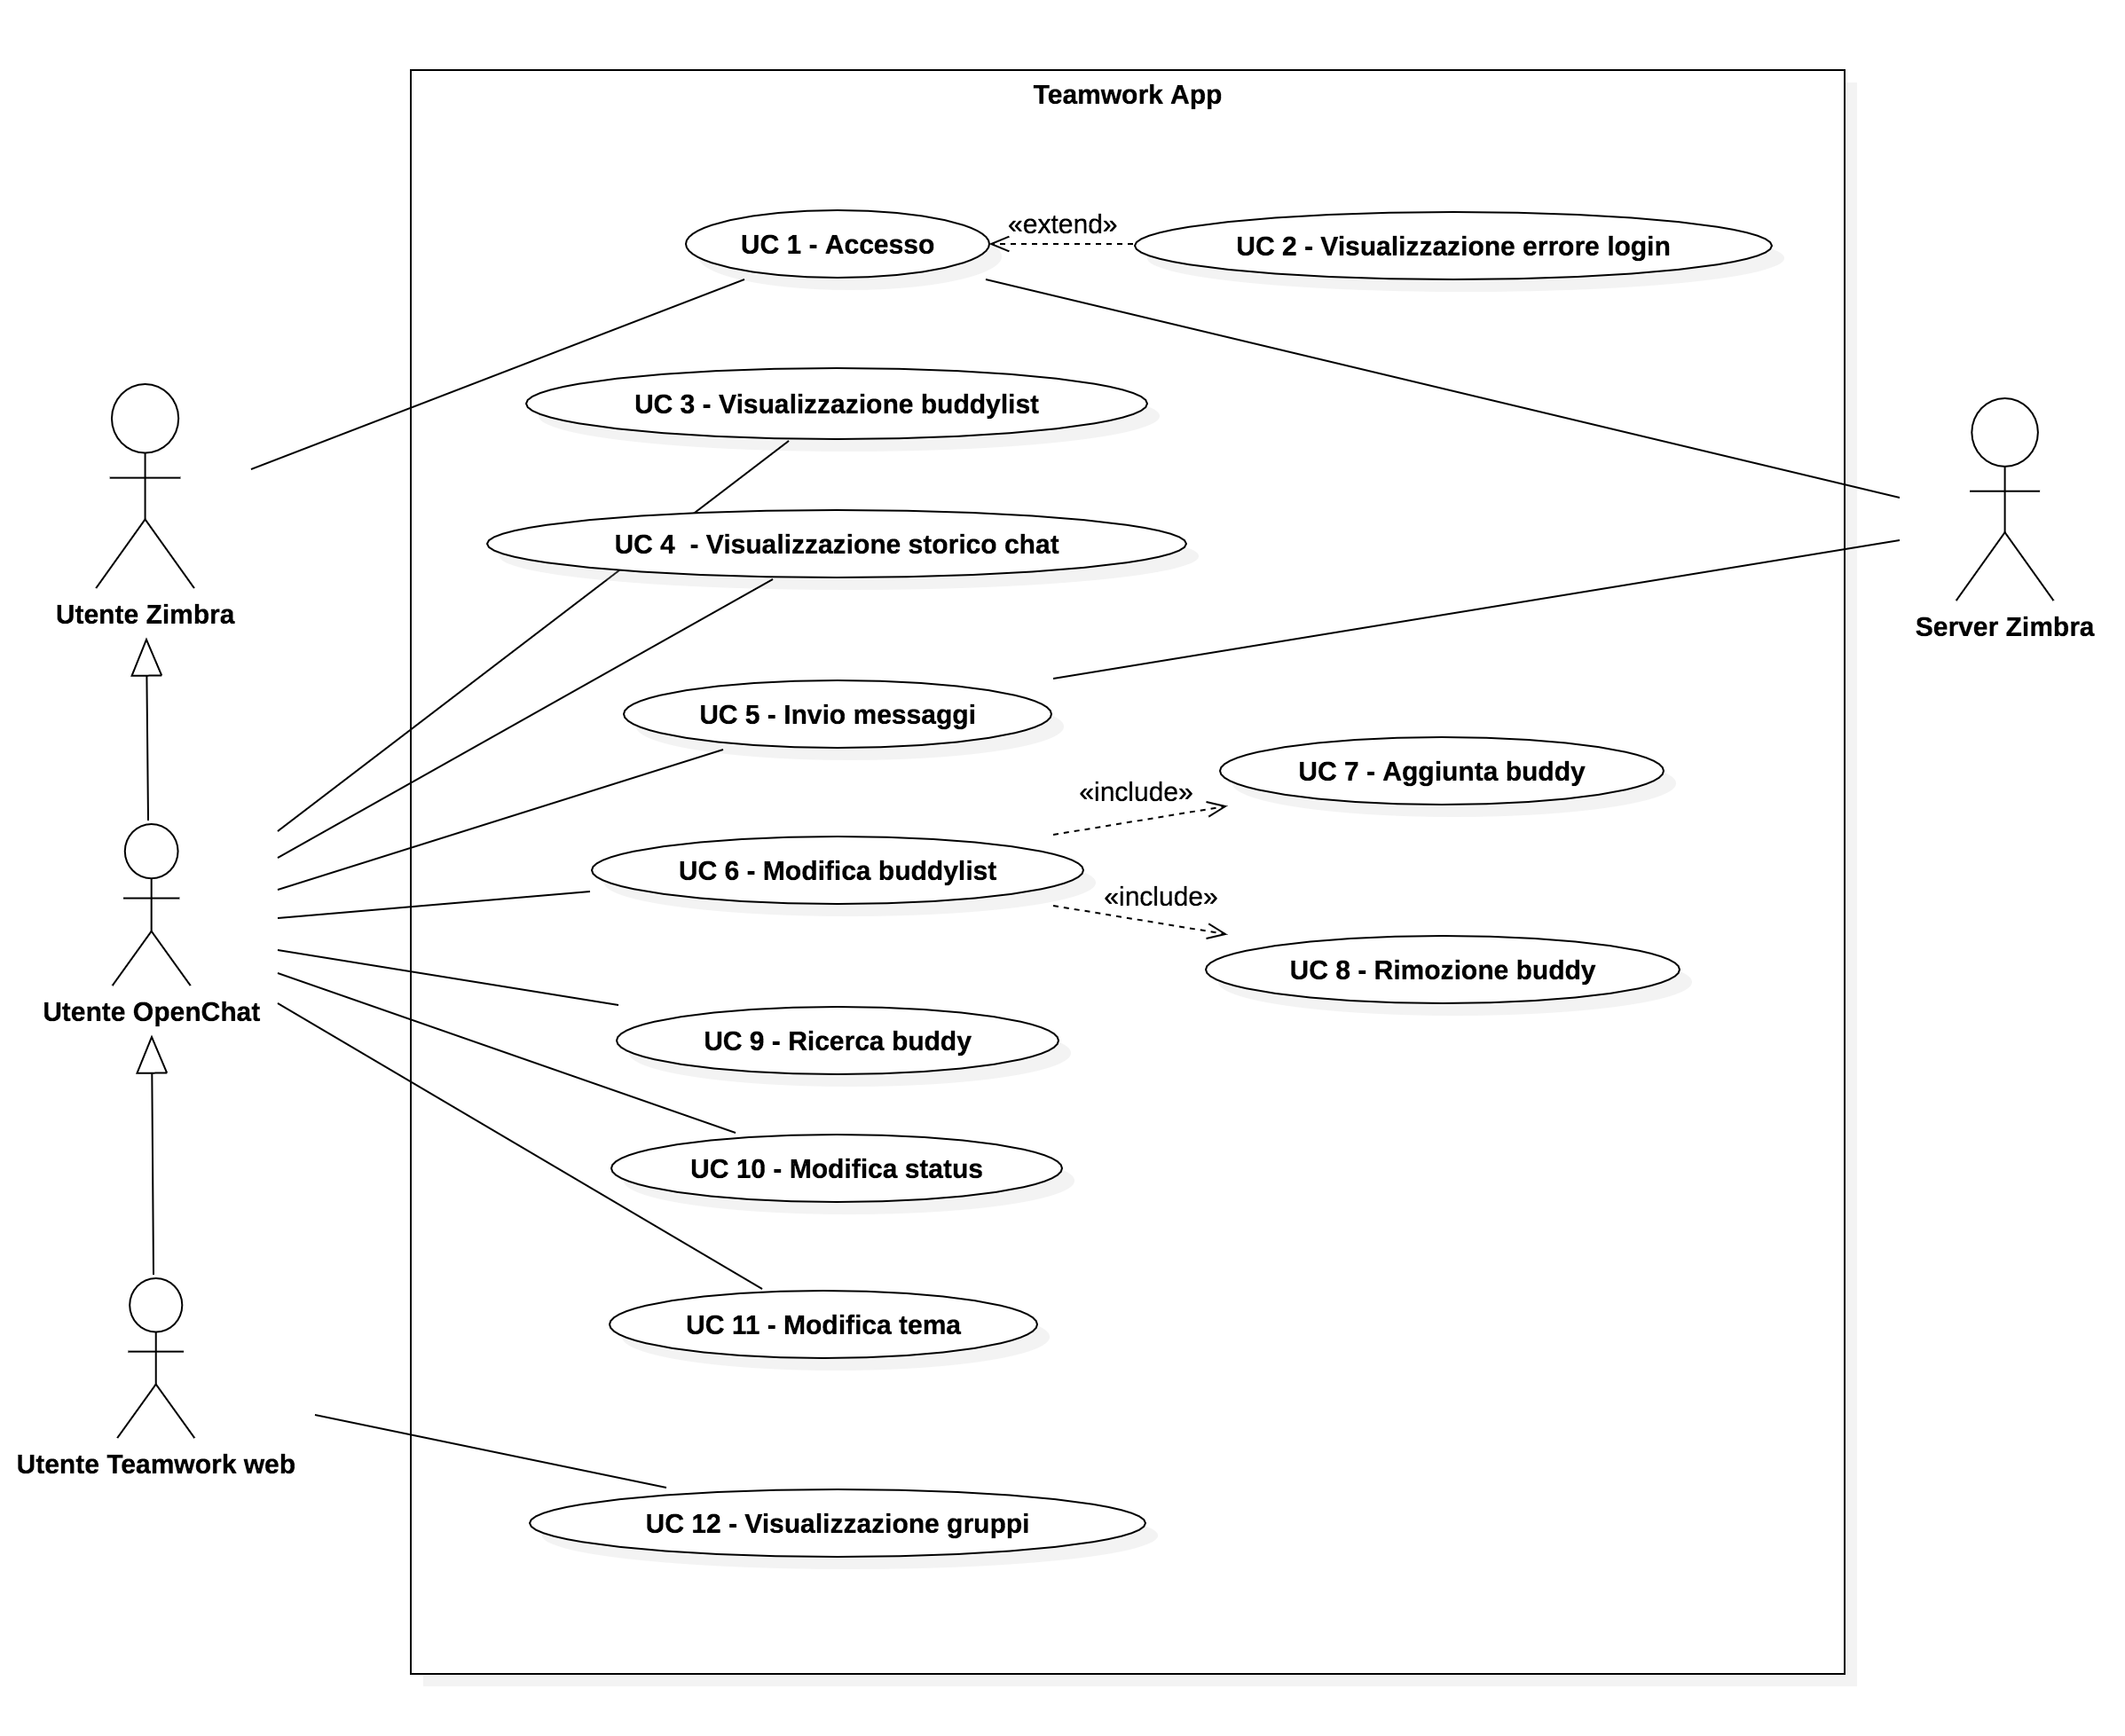
\includegraphics[scale=0.17]{UC/UCG}
		\caption{UCG - Caso d'uso generale}
	\end{figure}
	\begin{center}
	\bgroup
	\def\arraystretch{1.8}     
	\begin{longtable}{  p{4cm} | p{9.5cm} } 
		\textbf{Attori Primari} & Utente Zimbra, utente OpenChat e utente Teamwork web \\ 
		\textbf{Descrizione} & L'utente, se dispone della zimlet OpenChat potrà interagire con l'applicazione avendo modo di gestire e contattare la sua buddylist. Se nei suoi server Zimbra dispone della zimlet Teamwork web potrà interagire anche con i gruppi di cui fa parte. \\ 
		\textbf{Precondizioni}  & Il sistema è avviato e connesso a dei server Zimbra pronti per l'autenticazione; \\
		\textbf{Postcondizioni} & Il sistema ha eseguito tutte le funzioni richieste dall' attore permettendogli così di interagire con la sua buddylist e con i gruppi di cui fa parte  \\ 
		\textbf{Scenario principale} & 
		1. L’utente Zimbra vuole accedere all'applicazione Teamwork per mobile per gestire e comunicare con la sua lista contatti e con i gruppi;\newline
		2. L’utente OpenChat ha a disposizione la buddylist con le relative chat in modo da gestire nel modo che crede opportuno la comunicazione con i suoi buddy.
	\end{longtable}
	\egroup
\end{center}

% ---------------------------------------------------------------------------- %
\subsection{UC1 - Accesso}
	\begin{figure}[H] 
		\centering
		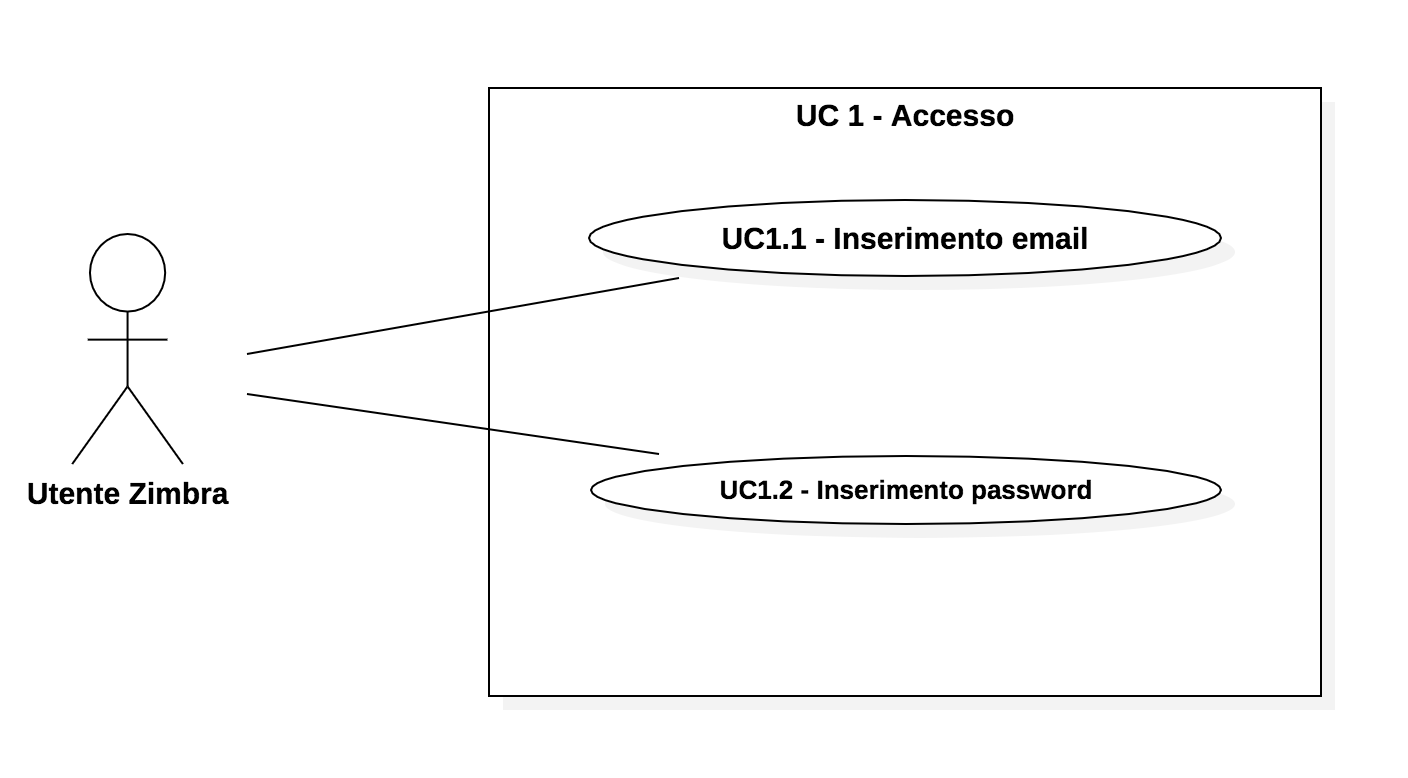
\includegraphics[scale=0.17]{UC/UC1}
		\caption{UC1 - Accesso}
	\end{figure}
	\begin{center}
	\bgroup
	\def\arraystretch{1.8}     
	\begin{longtable}{  p{4cm} | p{9.5cm} } 
		\textbf{Attori Primari} & Utente Zimbra; \\ 
		\textbf{Descrizione} & L’attore si può autenticare inserendo l'e-mail e la password con cui è registrato al server Zimbra; \\ 
		\textbf{Precondizioni}  & Il sistema è avviato, pronto per l’utilizzo e mostra la pagina di login; \\
		\textbf{Postcondizioni} & Il sistema ha autenticato l’attore e gli mostra la sua area riservata;  \\ 
		\textbf{Scenario principale} & 
			1. L’attore inserisce l'e-mail con cui è registrato al server Zimbra); \newline
			2. L’attore inserisce la sua password; \newline
			3. L’attore conferma il login e accede alla sua area riservata.\\
		\textbf{Estensioni} & Visualizzazione errore login (\ref{UC2}).
	\end{longtable}
	\egroup
\end{center}

\subsection{UC1.1 - Inserimento email}
	\begin{center}
	\bgroup
	\def\arraystretch{1.8}     
	\begin{longtable}{  p{4cm} | p{9.5cm} } 
		\textbf{Attori Primari} & Utente Zimbra; \\ 
		\textbf{Descrizione} & L’attore si può autenticare inserendo l'e-mail con cui è registrato al server Zimbra; \\ 
		\textbf{Precondizioni}  & Il sistema è avviato, pronto per l’utilizzo e mostra la pagina di login; \\
		\textbf{Postcondizioni} & Il sistema resta in attesa dell'inserimento della password da parte dell'attore per continuare l'autenticazione;  \\ 
		\textbf{Scenario principale} & 
		1. L’attore inserisce l'e-mail con cui è registrato al server Zimbra).
	\end{longtable}
	\egroup
\end{center}
\subsection{UC1.2 - Inserimento password}
	\begin{center}
	\bgroup
	\def\arraystretch{1.8}     
	\begin{longtable}{  p{4cm} | p{9.5cm} } 
		\textbf{Attori Primari} & Utente Zimbra; \\ 
		\textbf{Descrizione} & L’attore si può autenticare inserendo la password del profilo Zimbra; \\ 
		\textbf{Precondizioni}  & Il sistema è avviato, pronto per l’utilizzo e mostra la pagina di login; \\
		\textbf{Postcondizioni} & Il sistema resta in attesa della conferma da parte dell'attore per continuare l'autenticazine;  \\ 
		\textbf{Scenario principale} & 
		1. L’attore inserisce la sua password.
	\end{longtable}
	\egroup
\end{center}
% ---------------------------------------------------------------------------- %

\subsection{UC2 - Visualizzazione errore login} \label{UC2}
	\begin{center}
	\bgroup
	\def\arraystretch{1.8}     
	\begin{longtable}{  p{4cm} | p{9.5cm} } 
		\textbf{Attori Primari} & Utente Zimbra; \\ 
		\textbf{Descrizione} &  L'attore visualizza un messaggio di errore in quanto le credenziali da lui inserite non sono corrette; \\ 
		\textbf{Precondizioni}  & L'attore ha cercato di effettuare il login inserendo delle credenziali errate; \\
		\textbf{Postcondizioni} & L'attore ha visualizzato il messaggio di errore;  \\ 
		\textbf{Scenario principale} & 
		1. L'attore prova ad autenticarsi inserendo delle credenziali errate; \newline
		2. L'attore visualizza il messaggio di errore;
	\end{longtable}
	\egroup
\end{center}

% ---------------------------------------------------------------------------- %

\subsection{UC3 - Visualizzazione buddylist}
	\begin{figure}[H] 
	\centering
	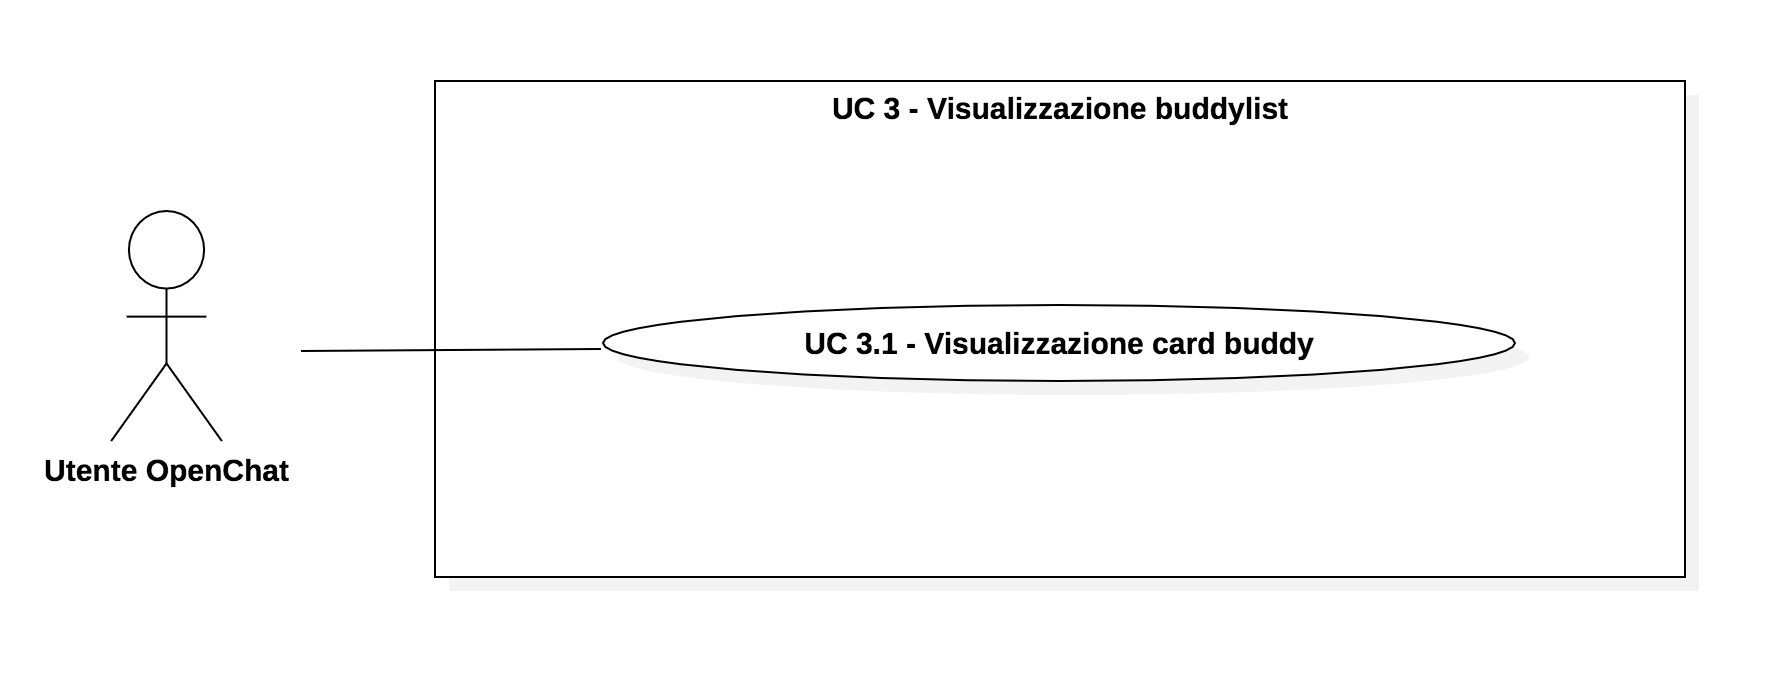
\includegraphics[scale=0.17]{UC/UC3}
	\caption{UC3 - Visualizzazione buddylist}
\end{figure}
	\begin{center}
	\bgroup
	\def\arraystretch{1.8}     
	\begin{longtable}{  p{4cm} | p{9.5cm} } 
		\textbf{Attori Primari} & Utente OpenChat; \\ 
		\textbf{Descrizione} &  L'attore può visualizzare l'intera lista dei buddy presenti nella sua buddylist; \\ 
		\textbf{Precondizioni}  & Talkapp presenta all'attore una pagina contenente la lista dei suoi buddy; \\
		\textbf{Postcondizioni} & L'attore ha visualizzato la lista dei suoi buddy;  \\ 
		\textbf{Scenario principale} & 
		1. L'attore seleziona l'icona nella tab riguardante la buddylist; \newline
		2. L'attore visualizza la buddylist contenente tutti i suoi buddy;
	\end{longtable}
	\egroup
\end{center}

\subsection{UC3.1 - Visualizzazione card buddy}
	\begin{figure}[H] 
	\centering
	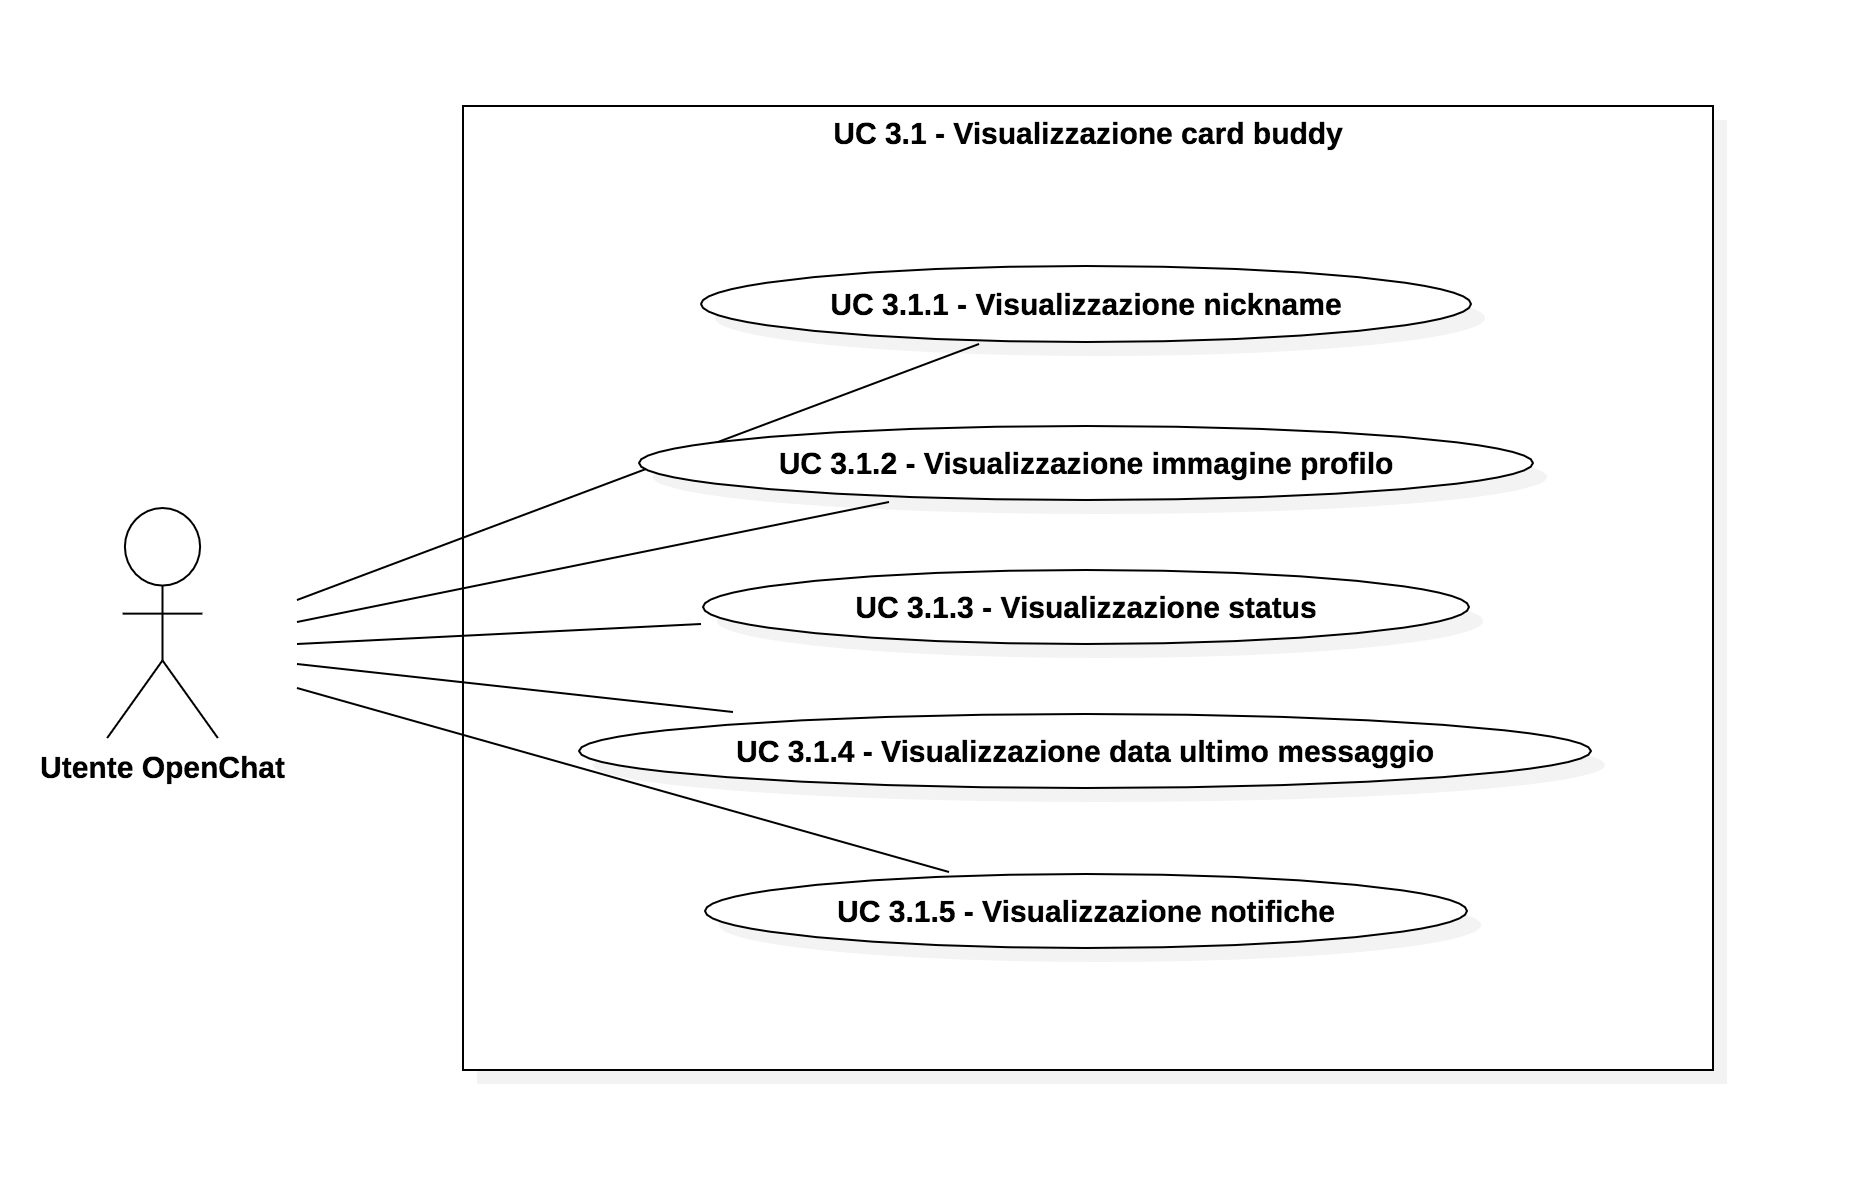
\includegraphics[scale=0.17]{UC/UC3_1}
	\caption{UC3.1 - Visualizzazione card buddy}
\end{figure}
		\begin{center}
		\bgroup
		\def\arraystretch{1.8}     
		\begin{longtable}{  p{4cm} | p{9.5cm} } 
			\textbf{Attori Primari} & Utente OpenChat; \\ 
			\textbf{Descrizione} &  L'attore può visualizzare dei dati significativi di ogni buddy presente nella sua buddylist; \\ 
			\textbf{Precondizioni}  & Talkapp presenta all'attore una pagina contenente la lista dei suoi buddy; \\
			\textbf{Postcondizioni} & L'attore ha visualizzato per ogni buddy una card contenente dei dettagli;  \\ 
			\textbf{Scenario principale} & 
			1. L'attore seleziona l'icona nella tab riguardante la buddylist; \newline
			2. L'attore visualizza per ogni buddy una card in cui sono presenti dei dettagli;
		\end{longtable}
		\egroup
	\end{center}

\subsection{UC3.1.1 - Visualizzazione nickname}
	\begin{center}
	\bgroup
	\def\arraystretch{1.8}     
	\begin{longtable}{  p{4cm} | p{9.5cm} } 
		\textbf{Attori Primari} & Utente OpenChat; \\ 
		\textbf{Descrizione} &  L'attore può visualizzare il nickname dato ad un buddy della sua buddylist; \\ 
		\textbf{Precondizioni}  & Talkapp presenta all'attore una pagina contenente la lista dei suoi buddy; \\
		\textbf{Postcondizioni} & L'attore ha visualizzato per ogni buddy il nickname dato;  \\ 
		\textbf{Scenario principale} & 
		1. L'attore seleziona l'icona nella tab riguardante la buddylist; \newline
		2. L'attore visualizza il nickname del buddy nella card a esso collegata;
	\end{longtable}
	\egroup
\end{center}
\subsection{UC3.1.2 - Visualizzazione immagine profilo}
	\begin{center}
	\bgroup
	\def\arraystretch{1.8}     
	\begin{longtable}{  p{4cm} | p{9.5cm} } 
		\textbf{Attori Primari} & Utente OpenChat; \\ 
		\textbf{Descrizione} &  L'attore può visualizzare l'immagine profilo di ogni buddy della sua buddylist; \\ 
		\textbf{Precondizioni}  & Talkapp presenta all'attore una pagina contenente la lista dei suoi buddy; \\
		\textbf{Postcondizioni} & L'attore ha visualizzato per ogni buddy  l'immagine profilo;  \\ 
		\textbf{Scenario principale} & 
		1. L'attore seleziona l'icona nella tab riguardante la buddylist; \newline
		2. L'attore visualizza l'immagine profilo del buddy nella card a esso collegata;
	\end{longtable}
	\egroup
\end{center}
\subsection{UC3.1.3 - Visualizzazione status}
	\begin{center}
		\bgroup
		\def\arraystretch{1.8}     
		\begin{longtable}{  p{4cm} | p{9.5cm} } 
			\textbf{Attori Primari} & Utente OpenChat; \\ 
			\textbf{Descrizione} &  L'attore può visualizzare lo status di ogni buddy della sua buddylist; \\ 
			\textbf{Precondizioni}  & Talkapp presenta all'attore una pagina contenente la lista dei suoi buddy; \\
			\textbf{Postcondizioni} & L'attore ha visualizzato per ogni buddy  il loro status;  \\ 
			\textbf{Scenario principale} & 
			1. L'attore seleziona l'icona nella tab riguardante la buddylist; \newline
			2. L'attore visualizza lo status del buddy nella card a esso collegata;
		\end{longtable}
		\egroup
	\end{center}
\subsection{UC3.1.4 - Visualizzazione data ultimo messaggio}
	\begin{center}
		\bgroup
		\def\arraystretch{1.8}     
		\begin{longtable}{  p{4cm} | p{9.5cm} } 
			\textbf{Attori Primari} & Utente OpenChat; \\ 
			\textbf{Descrizione} &  L'attore può visualizzare la data dell'ultimo messaggio scambiato con un particolare buddy della propria buddylist; \\ 
			\textbf{Precondizioni}  & Talkapp presenta all'attore una pagina contenente la lista dei suoi buddy; \\
			\textbf{Postcondizioni} & L'attore ha visualizzato per ogni buddy  la data dell'ultimo messaggio scambiato con esso;  \\ 
			\textbf{Scenario principale} & 
			1. L'attore seleziona l'icona nella tab riguardante la buddylist; \newline
			2. L'attore visualizza la data dell'ultimo messaggio scambiato con un buddy nella card a esso collegata;
		\end{longtable}
		\egroup
	\end{center}
\subsection{UC3.1.5 - Visualizzazione notifiche}
	\begin{center}
		\bgroup
		\def\arraystretch{1.8}     
		\begin{longtable}{  p{4cm} | p{9.5cm} } 
			\textbf{Attori Primari} & Utente OpenChat; \\ 
			\textbf{Descrizione} &  L'attore può visualizzare il numero dei messaggi ricevuti da un particolare buddy della sua buddylist e non ancora letti; \\ 
			\textbf{Precondizioni}  & Talkapp presenta all'attore una pagina contenente la lista dei suoi buddy; \\
			\textbf{Postcondizioni} & L'attore ha visualizzato per ogni buddy il numero dei messaggi ricevuti da esso e non ancora letti;  \\ 
			\textbf{Scenario principale} & 
			1. L'attore seleziona l'icona nella tab riguardante la buddylist; \newline
			2. L'attore visualizza il numero dei messaggi ricevuto da un particolare buddy e non ancora letti nella card a esso collegata;
		\end{longtable}
		\egroup
	\end{center}

% ---------------------------------------------------------------------------- %

\subsection{UC4 - Visualizzazione storico chat}
	\begin{figure}[H] 
	\centering
	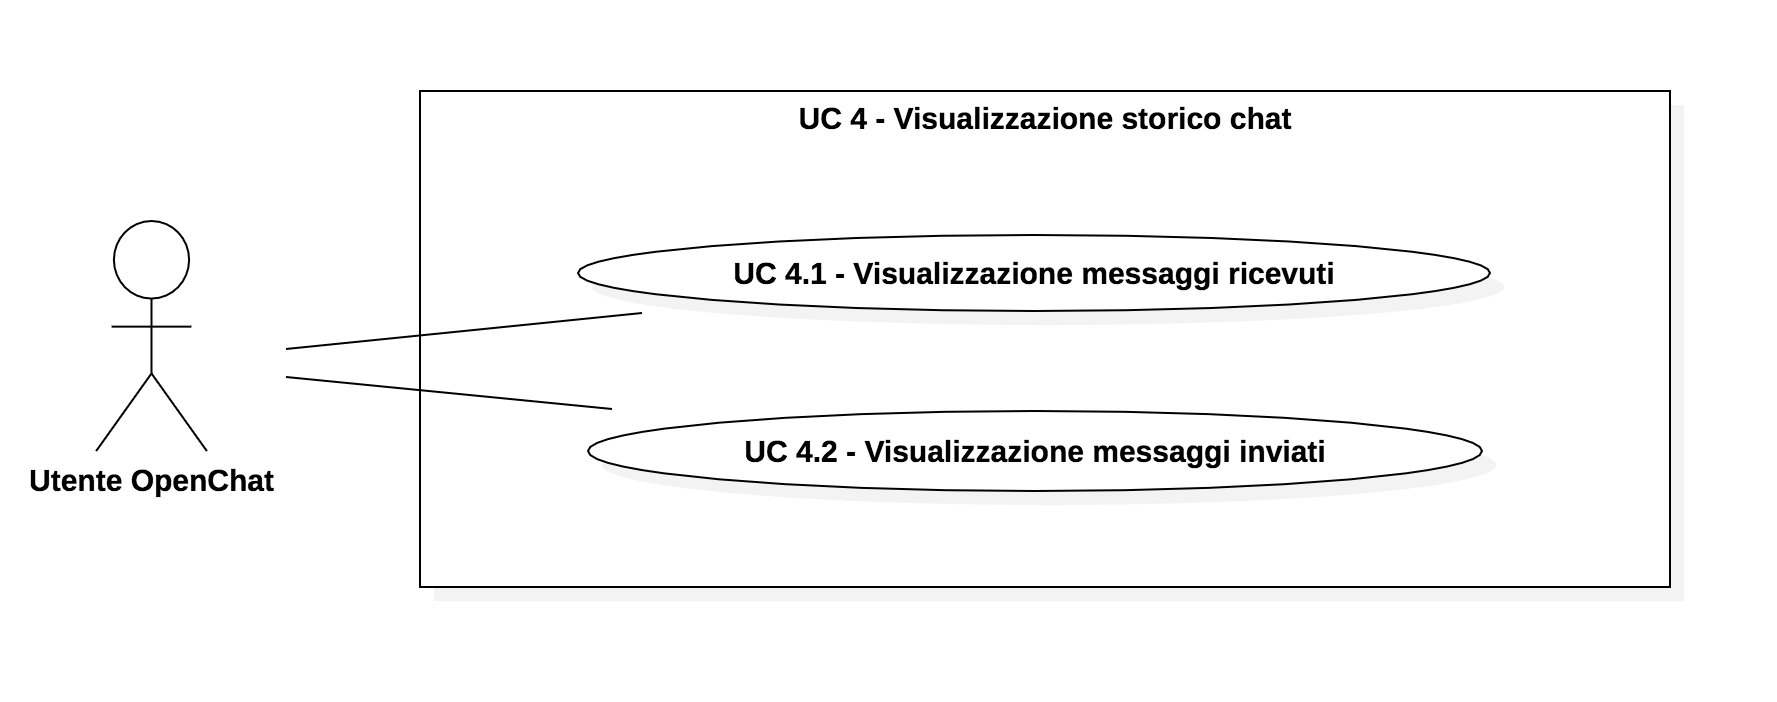
\includegraphics[scale=0.17]{UC/UC4}
	\caption{UC4 - Visualizzazione storico chat}
\end{figure}
	\begin{center}
	\bgroup
	\def\arraystretch{1.8}     
	\begin{longtable}{  p{4cm} | p{9.5cm} } 
		\textbf{Attori Primari} & Utente OpenChat; \\ 
		\textbf{Descrizione} &  L'attore può visualizzare lo storico delle conversazioni avute con i suoi buddy; \\ 
		\textbf{Precondizioni}  & Talkapp presenta all'attore una pagina contenente la lista dei suoi buddy; \\
		\textbf{Postcondizioni} & L'attore ha visualizzato la lista dei messaggi scambiati con un particolare buddy;  \\ 
		\textbf{Scenario principale} & 
		1. L'attore seleziona un buddy dalla sua buddylist; \newline
		2. L'attore visualizza la lista dei messaggi scambiati nel tempo con il buddy selezionato;
	\end{longtable}
	\egroup
\end{center}

\subsection{UC4.1 - Visualizzazione messaggi ricevuti}
	\begin{center}
	\bgroup
	\def\arraystretch{1.8}     
	\begin{longtable}{  p{4cm} | p{9.5cm} } 
		\textbf{Attori Primari} & Utente OpenChat; \\ 
		\textbf{Descrizione} &  L'attore può visualizzare i messaggi ricevuti da un particolare buddy; \\ 
		\textbf{Precondizioni}  & Talkapp presenta all'attore una pagina contenente la lista dei suoi buddy; \\
		\textbf{Postcondizioni} & L'attore ha visualizzato la lista dei messaggi ricevuti  da un particolare buddy;  \\ 
		\textbf{Scenario principale} & 
		1. L'attore seleziona un buddy dalla sua buddylist; \newline
		2. L'attore visualizza la lista dei messaggi ricevuti nel tempo dal buddy selezionato;
	\end{longtable}
	\egroup
\end{center}

\subsection{UC4.2 - Visualizzazione messaggi inviati}
	\begin{center}
	\bgroup
	\def\arraystretch{1.8}     
	\begin{longtable}{  p{4cm} | p{9.5cm} } 
		\textbf{Attori Primari} & Utente OpenChat; \\ 
		\textbf{Descrizione} &  L'attore può visualizzare i messaggi inviati ad un particolare buddy; \\ 
		\textbf{Precondizioni}  & Talkapp presenta all'attore una pagina contenente la lista dei suoi buddy; \\
		\textbf{Postcondizioni} & L'attore ha visualizzato la lista dei messaggi inviati  ad un particolare buddy;  \\ 
		\textbf{Scenario principale} & 
		1. L'attore seleziona un buddy dalla sua buddylist; \newline
		2. L'attore visualizza la lista dei messaggi inviati nel tempo al buddy selezionato;
	\end{longtable}
	\egroup
\end{center}

% ---------------------------------------------------------------------------- %

\subsection{UC5 - Invio messaggi}
	\begin{center}
	\bgroup
	\def\arraystretch{1.8}     
	\begin{longtable}{  p{4cm} | p{9.5cm} } 
		\textbf{Attori Primari} & Utente OpenChat; \\ 
		\textbf{Descrizione} &  L'attore può inviare messaggi ad un buddy; \\ 
		\textbf{Precondizioni}  & Talkapp presenta all'attore una pagina contenente lo storico delle conversazioni avute con un particolare buddy; \\
		\textbf{Postcondizioni} & L'attore ha inviato un messaggio ad un buddy; \\ 
		\textbf{Scenario principale} & 
		1. L'attore seleziona un buddy dalla sua buddylist; \newline
		2. L'attore digita un messaggio nel box apposito; \newline
		3. L'attore preme il pulsante di fianco al box per confermare l'invio;
		4. Il messaggio appare nello storico della chat.
	\end{longtable}
	\egroup
\end{center}

\subsection{UC6 - Modifica buddylist}
	\begin{center}
	\bgroup
	\def\arraystretch{1.8}     
	\begin{longtable}{  p{4cm} | p{9.5cm} } 
		\textbf{Attori Primari} & Utente OpenChat; \\ 
		\textbf{Descrizione} &  L'attore può modificare la buddylist visualizzata; \\ 
		\textbf{Precondizioni}  & Talkapp presenta all'attore una pagina contenente la lista dei suoi buddy \\
		\textbf{Postcondizioni} & L'attore ha modificato la buddylist che viene visualizzata; \\ 
		\textbf{Scenario principale} & 
		1. L'attore seleziona un buddy da rimuovere o digita un contatto da aggiungere; \newline
		2. L'attore conferma di voler cambiate la buddylist tramite l''azione svolta;
	\end{longtable}
	\egroup
\end{center}

\subsection{UC7 - Aggiunta buddy}
	\begin{center}
	\bgroup
	\def\arraystretch{1.8}     
	\begin{longtable}{  p{4cm} | p{9.5cm} } 
		\textbf{Attori Primari} & Utente OpenChat; \\ 
		\textbf{Descrizione} &  L'attore può aggiungere un nuovo buddy alla sua buddylist; \\ 
		\textbf{Precondizioni}  & Talkapp presenta all'attore una pagina contenente un form per l'aggiunta di un buddy; \\
		\textbf{Postcondizioni} & L'attore ha aggiunto un buddy alla sua buddylist;  \\ 
		\textbf{Scenario principale} & 
		1. L'attore inserisce il nickname che vuole dare al buddy; \newline
		2. L'attore inserisce l'e-mail del buddy che vuole aggiungere; \newline
		3. L'attore conferma l'aggiunta del buddy alla propria buddylist.
	\end{longtable}
	\egroup
\end{center}

\subsection{UC8 - Rimozione buddy}
	\begin{center}
	\bgroup
	\def\arraystretch{1.8}     
	\begin{longtable}{  p{4cm} | p{9.5cm} } 
		\textbf{Attori Primari} & Utente OpenChat; \\ 
		\textbf{Descrizione} &  L'attore può rimuovere un buddy dalla sua buddylist; \\ 
		\textbf{Precondizioni}  & Talkapp presenta all'attore una pagina contenente i dettagli del buddy selezionato e le azioni che possono essere svolte; \\
		\textbf{Postcondizioni} & L'attore ha rimosso il buddy dalla sua buddylist;  \\ 
		\textbf{Scenario principale} & 
		1. L'attore seleziona il buddiy dalla buddylist che vuole rimuovere; \newline
		2. L'attore seleziona la voce "Rimozione" dal menù di azioni disponibili; \newline
		3. L'attore conferma la rimozione del buddy dalla propria buddylist.
	\end{longtable}
	\egroup
\end{center}

\subsection{UC9 - Ricerca buddy}
	\begin{center}
	\bgroup
	\def\arraystretch{1.8}     
	\begin{longtable}{  p{4cm} | p{9.5cm} } 
		\textbf{Attori Primari} & Utente OpenChat; \\ 
		\textbf{Descrizione} &  L'attore può ricercare un  buddy tra quelli presenti nella sua buddylist; \\ 
		\textbf{Precondizioni}  & Talkapp presenta all'attore una pagina contenente un campo di ricerca per ricercare un buddy in base ad un certo testo; \\
		\textbf{Postcondizioni} & L'attore ha ricercato un buddy dalla sua buddylist in base ad un testo da lui inserito;  \\ 
		\textbf{Scenario principale} & 
		1. L'attore inserisce dei caratteri nel campo di ricerca; \newline
		2. L'attore visualizza i buddy corrispondenti alla ricerca da lui effettuata;
	\end{longtable}
	\egroup
\end{center}

\subsection{UC10 - Modifica status}
	\begin{center}
	\bgroup
	\def\arraystretch{1.8}     
	\begin{longtable}{  p{4cm} | p{9.5cm} } 
		\textbf{Attori Primari} & Utente OpenChat; \\ 
		\textbf{Descrizione} &  L'attore può modificare lo status con cui viene visualizzato dagli altri utenti; \\ 
		\textbf{Precondizioni}  & Talkapp presenta all'attore una pagina contenente un elenco degli statusdis ponibili; \\
		\textbf{Postcondizioni} & L'attore ha modificato lo status con cui viene visualizzato dagli altri utenti; \\ 
		\textbf{Scenario principale} & 
		1. L'attore seleziona uno status tra quelli disponibili; \newline
		2. L'attore conferma di voler cambiate status con quello selezionato;
	\end{longtable}
	\egroup
\end{center}

\subsection{UC11 - Modifica tema}
	\begin{center}
	\bgroup
	\def\arraystretch{1.8}     
	\begin{longtable}{  p{4cm} | p{9.5cm} } 
		\textbf{Attori Primari} & Utente OpenChat; \\ 
		\textbf{Descrizione} &  L'attore può modificare il tema dei colori con cui visualizza l'applicazione; \\ 
		\textbf{Precondizioni}  & Talkapp presenta all'attore una pagina contenente un elenco con tutti i temi disponibili; \\
		\textbf{Postcondizioni} & L'attore ha modificato il tema dell'applicazione; \\ 
		\textbf{Scenario principale} & 
		1. L'attore seleziona un tema tra quelli disponibili da applicare \newline
		2. L'attore conferma di voler applicare quel tema;
	\end{longtable}
	\egroup
\end{center}

\subsection{UC12 - Visualizzazione gruppi}
	\begin{center}
	\bgroup
	\def\arraystretch{1.8}     
	\begin{longtable}{  p{4cm} | p{9.5cm} } 
		\textbf{Attori Primari} & Utente Teamwork web; \\ 
		\textbf{Descrizione} &  L'attore può visualizzare l'elenco dei gruppi di cui fa parte; \\ 
		\textbf{Precondizioni}  & Talkapp presenta una pagina contenente i gruppi di cui fa parte; \\
		\textbf{Postcondizioni} & L'attore ha visualizzato i gruppi di cui fa parte; \\ 
		\textbf{Scenario principale} & 
		1. L'attore seleziona l'icona nella tab riguardante i gruppi; \newline
		2. L'attore visualizza i gruppi di cui fa parte;
	\end{longtable}
	\egroup
\end{center}



\section{Requisiti}
Ogni requisito qui riportato è identificato da un codice, ed è rappresentato nel seguente modo:
$$ \textbf{R \{importanza\}\{tipo\}\{numero\_vincolo\} } $$

\begin{itemize}
	\item "R" è prefisso di tutti i codici dei requisiti;
	\item Il primo valore rappresenta l'importanza: \textbf{0} se il requisito è obbligatorio, \textbf{1} se è desiderabile, \textbf{2} per gli opzionali;
	\item Il terzo valore indica il tipo: \textbf{F} per i requisiti funzionali, \textbf{Q} per quelli di qualità, \textbf{P} se prestazionale, \textbf{V} se di vincolo;
	\item L'ultimo numero indica il numero del vincolo. La struttura numerica di quest'ultimo rispetta le stesse regole dei Casi D'Uso.
\end{itemize}

\subsection{Principali requisiti funzionali}
\begin{longtable}{|c|c|}
	\hline
	\textbf{Id Requisito} & \textbf{Descrizione}\\
	\hline
	\endhead
	R0F1 & ....  \\ \hline 
	\caption{Requisiti di qualità}
	\label{tabella:req}
\end{longtable}

\subsection{Requisiti di vincolo}
\begin{longtable}{|c|c|}
	\hline
	\textbf{Id Requisito} & \textbf{Descrizione}\\
	\hline
	\endhead
	R0V1 & ....  \\ \hline 
	\caption{Requisiti di vincolo}
	\label{tabella:reqV}
\end{longtable}

\subsection{Requisiti di qualità}
\begin{longtable}{|c|c|}
	\hline
	\textbf{Id Requisito} & \textbf{Descrizione}\\
	\hline
	\endhead
	R0Q1 & ....  \\ \hline 
	\caption{Requisiti di qualità}
	\label{tabella:reqQ}
\end{longtable}

